\documentclass[10pt,aspectratio=169
	%,handout
	]{beamer}
	\usetheme[
	%%% options passed to the outer theme
	%   rotationcw,          % change the rotation direction from counter-clockwise to clockwise
		sectionpages, 		% show section pages
		logo={_figures/logo-federico-II-blue.png}
	]{UniNA}
	%\graphicspath{ {./images} }
	%\setbeamercovered{transparent}
	
	\usepackage[utf8]{inputenc}
	\usepackage[italian]{babel}
	\usepackage[T1]{fontenc}
	\usepackage{tikz}
	\usepackage{multimedia}

	\usepackage[scaled]{beramono}     %mono?
	\usepackage[scale=1.15]{AlegreyaSans}
	
	\title[Stabilizzazione nel piano di Gough-Stewart] %shown at the top of frames
	{\huge Stabilizzazione nel piano\\ di Gough-Stewart} %shown in title frame
	%\subtitle{M.Sc. Thesis in Computer Science}  % could also be a conference name
	
	%\date{December 6, 2018} %explicitly set date instead of \today
	
	\author[Daniele Facco]%shown at the top of frames
	{%shown in title frame
		{\footnotesize Presentato da}\\
		Daniele \textsc{Facco}%
	}
	
	% - Give the names in the same order as they appear in the paper.
	% - Use the \inst{?} command only if the authors have different
	%   affiliation. See the beamer manual for an example
	
	\institute[
		Dipartimento di ingegneria e architettura\\
		Università degli Studi di Trieste\\
		Italia
	]
	{% is placed on the bottom of the title page
		Università degli Studi di Trieste
	}

	\begin{document}

	\maketitle

	% TOC
	\begin{frame}{Argomenti trattati}{}
		\tableofcontents
	\end{frame}

	\section{Introduzione}
	% motivation for creating this theme
	\begin{frame}{Introduzione}{Piattaforma di Gough-Stewart}
		%\begin{block}{Why the UniNA beamer theme?}

	\begin{columns}
	\column{0.3\textwidth}
	%Stabilizzazione di una pallina su un piano mediante l'uso di una piattaforma di Gough-Stewart.
	
	\begin{itemize}
		\item Robot parallelo
		\item Esapode
		\item 6 gradi di libertà
		\item Attuatori rotativi
	\end{itemize}
	\column{0.7\textwidth}
	\centering 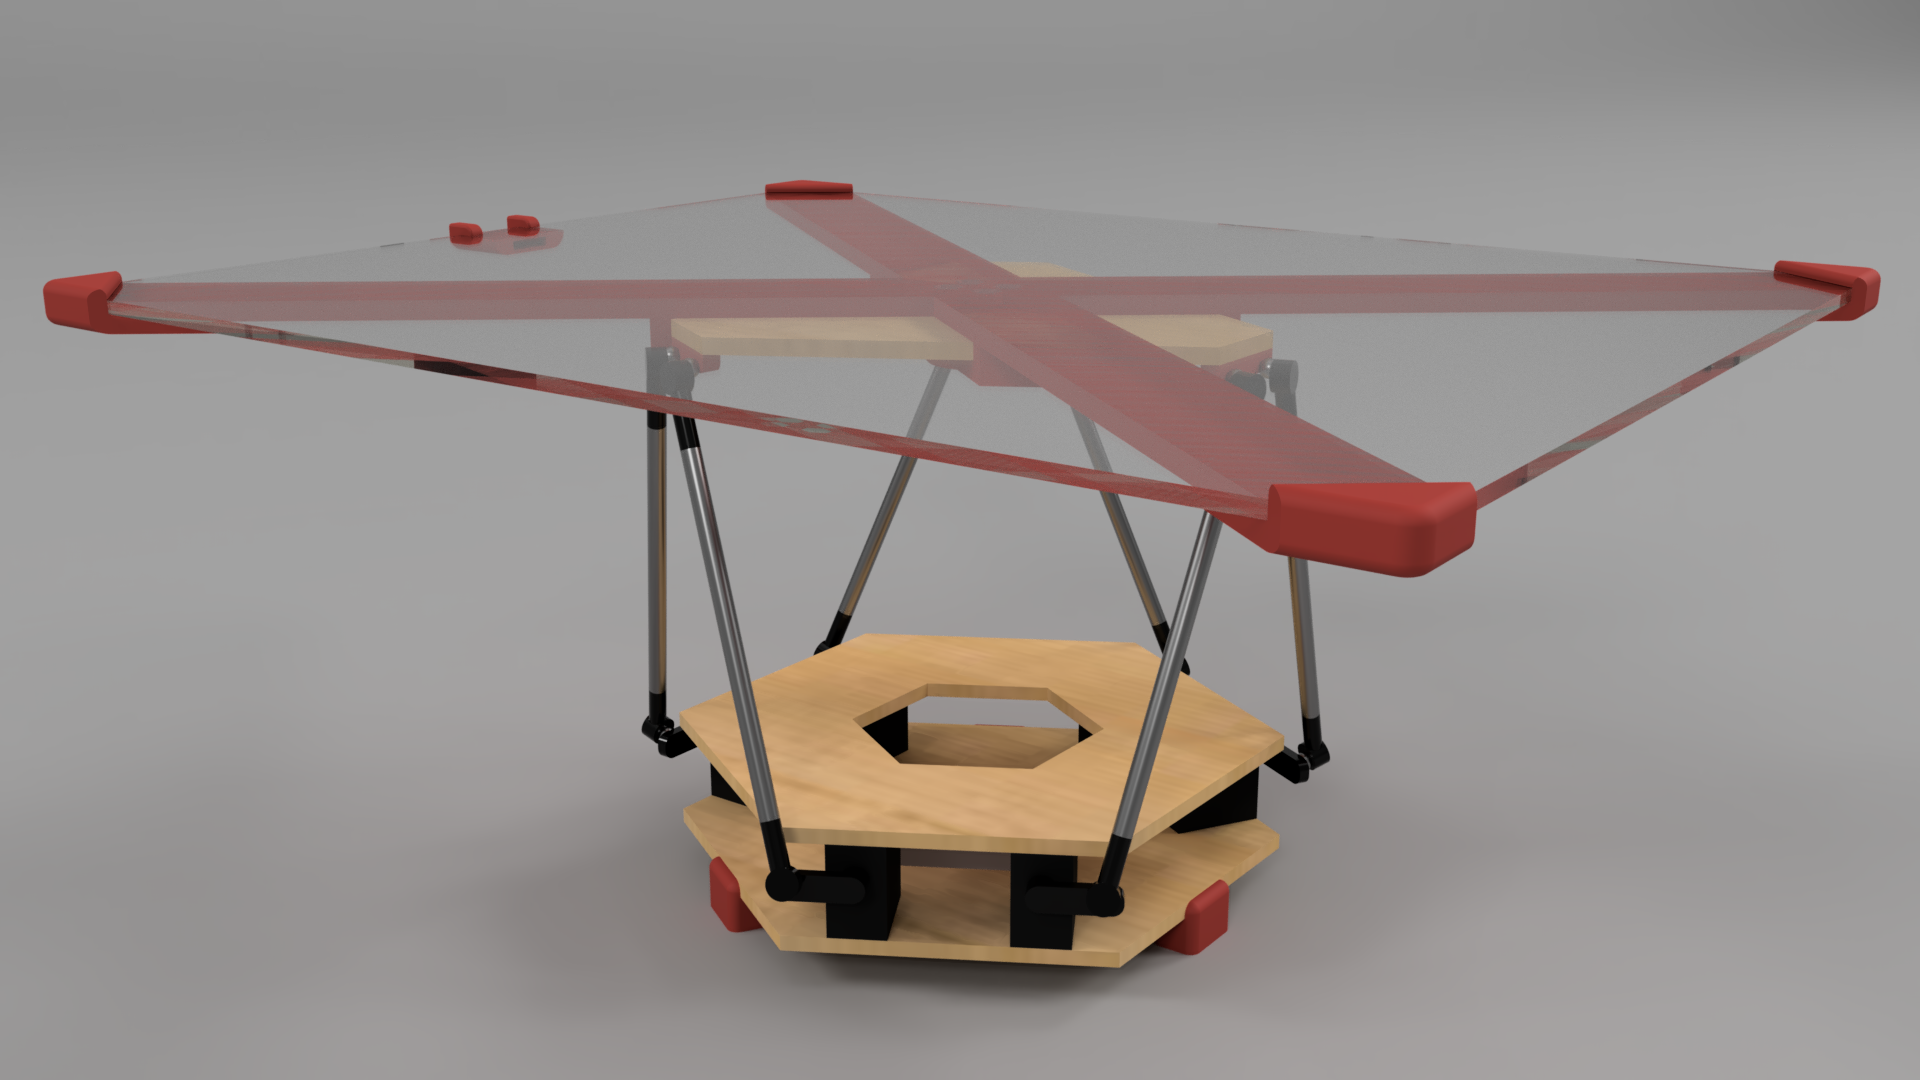
\includegraphics[width=\textwidth]{./images/stewart.png}
	\end{columns}
		%\end{block}
	\end{frame}
	
	\begin{frame}{Introduzione}{Tecnologie impiegate}
		%\begin{block}{Why the UniNA beamer theme?}

	\begin{columns}
	\column{0.3\textwidth}
	%Stabilizzazione di una pallina su un piano mediante l'uso di una piattaforma di Gough-Stewart.
	
	\begin{itemize}
		\item Arduino
		\item Servomotori
		\item Piano resistivo
		\item Ponte ad H
	\end{itemize}
	\column{0.7\textwidth}
	\centering 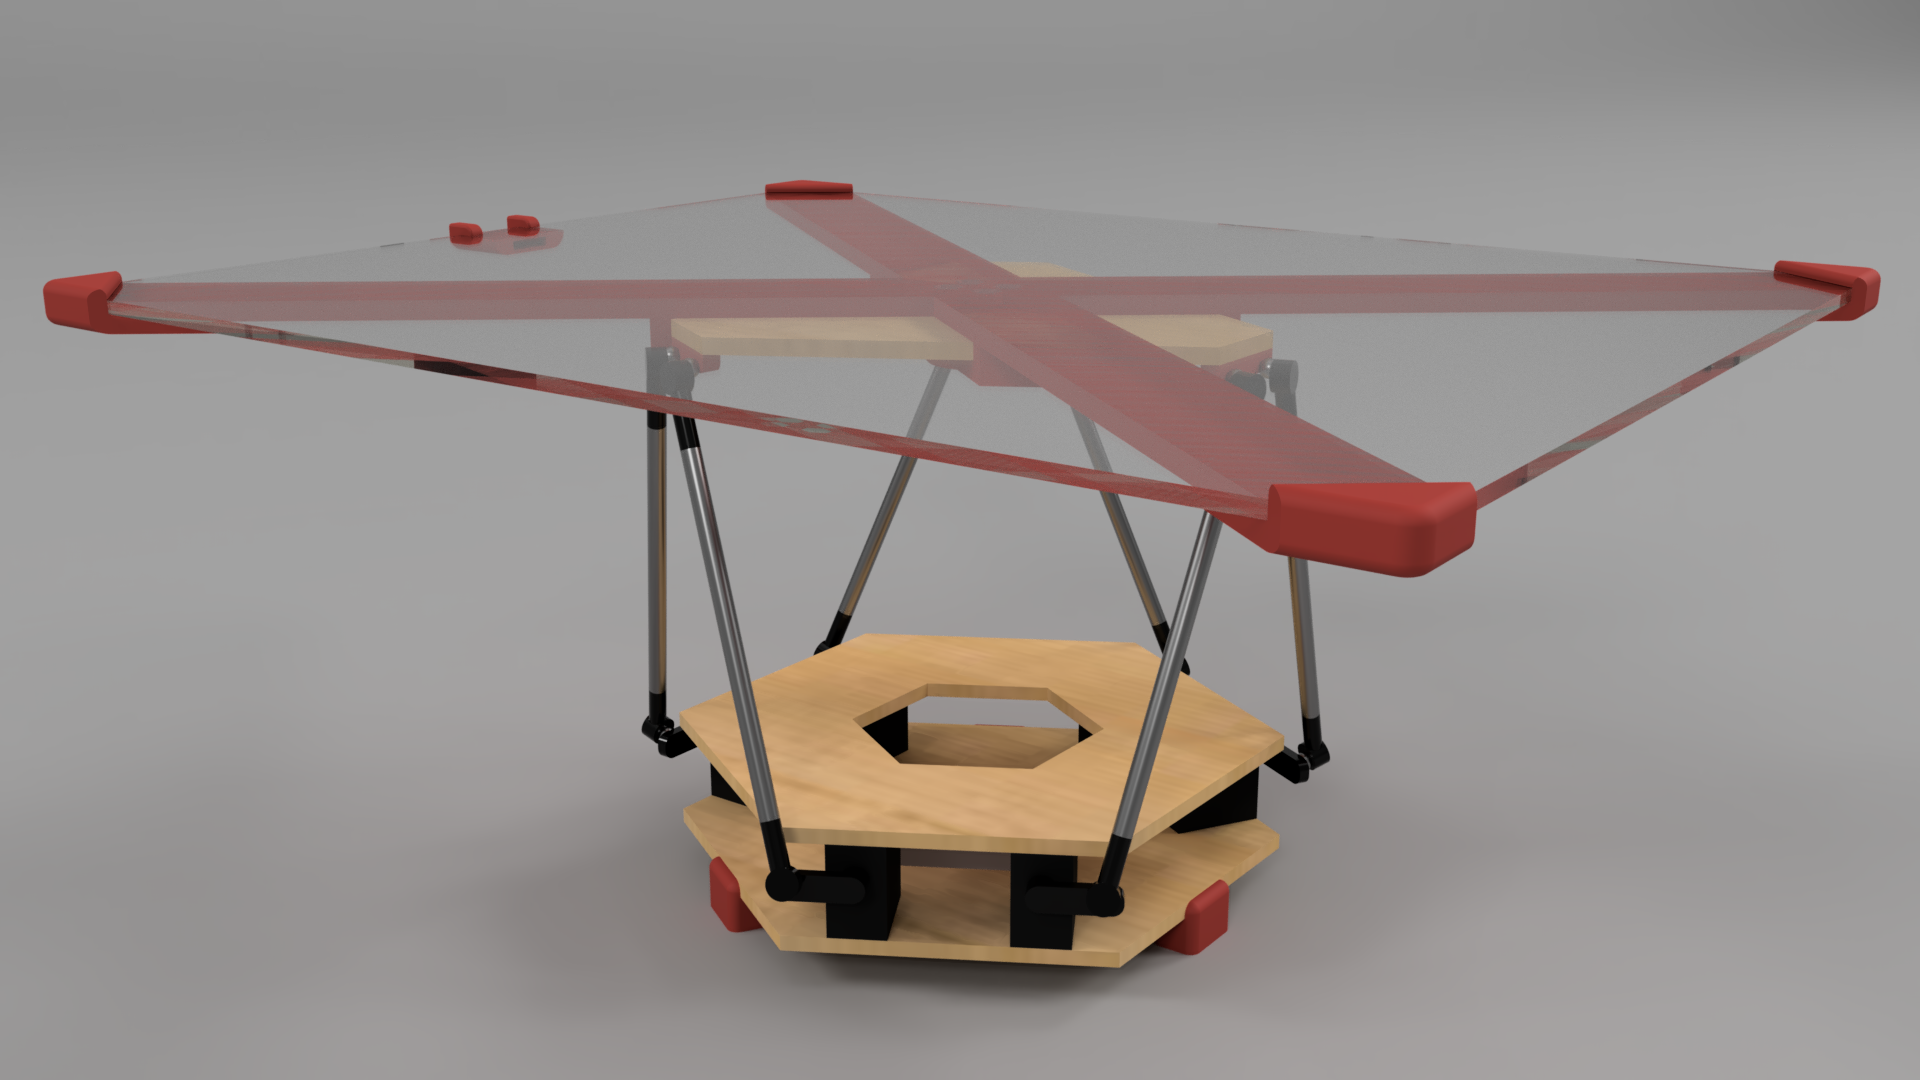
\includegraphics[width=\textwidth]{./images/stewart.png}
	\end{columns}
		%\end{block}
	\end{frame}
	
	\begin{frame}{Introduzione}{Realizzazione ponte ad H}

	\begin{columns}
	\column{0.3\textwidth}
	%Stabilizzazione di una pallina su un piano mediante l'uso di una piattaforma di Gough-Stewart.
	
	\begin{itemize}
		\item Arduino
		\item Servomotori
		\item Piano resistivo
		\item Ponte ad H
	\end{itemize}
	\column{0.7\textwidth}
	\centering
	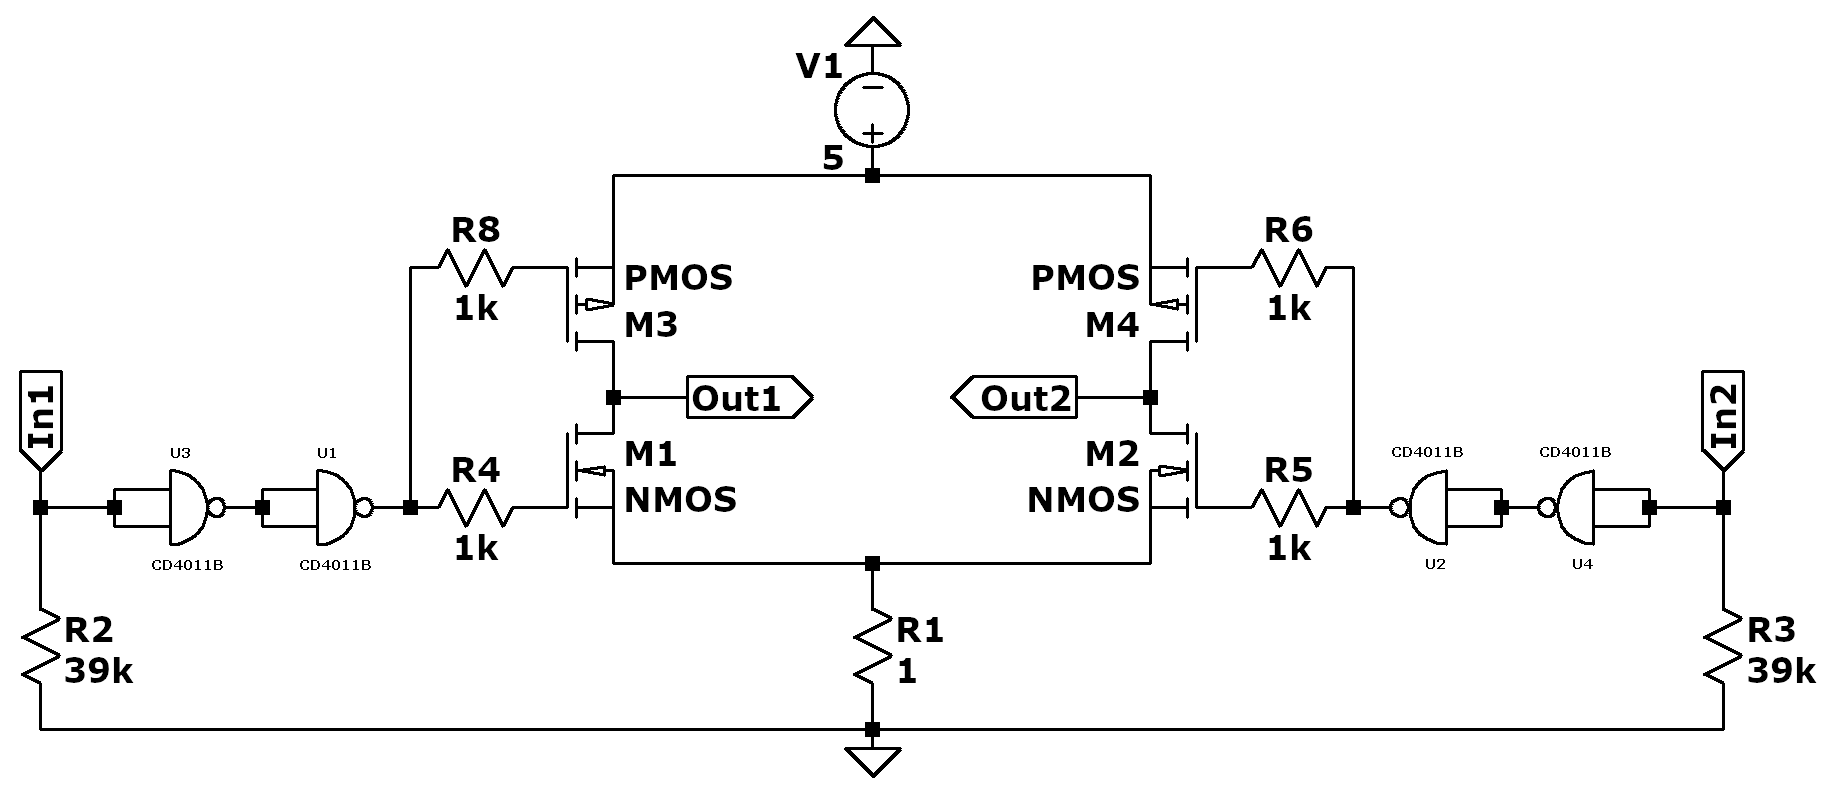
\includegraphics[width=\textwidth]{./images/circuit3.png}
	\end{columns}
		%\end{block}
	\end{frame}
	
	
	\section{Modello matematico}
	\subsection{Piattaforma di Gough-Stewart}
	\begin{frame}{Modello matematico}{Piattaforma di Gough-Stewart}

	\begin{columns}
	\column{0.4\textwidth}
	%Stabilizzazione di una pallina su un piano mediante l'uso di una piattaforma di Gough-Stewart.
	
	\begin{itemize}
		\item Analisi vettoriale
		\item Problema attuatori rotativi
		\item Angoli per raggiungere una posizione nello spazio
	\end{itemize}
	\column{0.6\textwidth}
	\centering
\scalebox{0.5}{
\begin{tikzpicture}
 
\filldraw[fill=yellow!50,rotate around={-10:(0,7cm)},xshift=2cm,yshift=1cm] (0,7cm) ellipse (4cm and 2cm);
\filldraw [fill=red!50](0,0) ellipse (5cm and 2.5cm);
\draw [-latex, thick] (0,0) -- node[anchor=south]{$\hat b_i$}(5cm,0);
\draw [-latex, thick] (0,0) -- node[anchor=east]{$\hat T$}(2.15cm,7.65cm);
\draw [-latex, thick] (0,0) -- node[anchor=north]{$\hat q_i$}(6.1cm,6.95cm);
\draw [-latex, thick] (5cm,0) -- node[anchor=west]{$\hat l_i$}(6.1cm,6.95cm);
\draw[-latex, thick,rotate around={-10:(0,7cm)},xshift=2cm,yshift=1cm] (0cm,7cm) -- node[anchor=south]{$\hat p_i$}(4cm,7cm);
\filldraw [fill=black] (0,0) circle (2pt) node[yshift= -0.25cm] {$O$} node[xshift= -2cm] {Base};
\filldraw [fill=black] (5cm,0) circle (2pt) node[anchor=west]{$B_i$};
\filldraw [fill=black] (2.15cm,7.65cm) circle (2pt) node[yshift= 0.25cm] {$O'$} node[xshift= -2cm] {Piattaforma};
\filldraw [fill=black] (6.1cm,6.95cm) circle (2pt) node[anchor=west]{$P_i$};
\draw [-latex, thick] (-1,-1.5) -- node[anchor=north]{$\hat i$}(0cm,-1.5cm);
\draw [-latex, thick] (-1,-1.5) -- node[anchor=east]{$\hat k$}(-1cm,-0.5cm);
\draw [-latex, thick,rotate around={-120:(-1,-1.5cm)}] (-1,-1.5) -- node[anchor=east]{$\hat j$}(-0.5cm,-1.5cm);

\draw [-latex, thick,rotate around={-10:(0,8.5cm)}] (0,8.5) -- node[anchor=north]{$\hat {i'}$}(1cm,8.5cm);
\draw [-latex, thick,rotate around={-10:(0,8.5cm)}] (0,8.5) -- node[anchor=east]{$\hat {k'}$}(0cm,9.5cm);
\draw [-latex, thick,rotate around={-130:(0,8.5cm)}] (0,8.5) -- node[anchor=east]{$\hat {j'}$}(0.5cm,8.5cm);

\end{tikzpicture}
}
	\end{columns}
		%\end{block}
	\end{frame}
	
	\begin{frame}{Modello matematico}{Piano inclinato e controllore PID}

	\begin{itemize}
		\item Funzione di trasferimento piano inclinato
		\item Controllore PID
		\item Analisi di stabilità
		\item Miglioramenti impiegati
	\end{itemize}
	\centering
\scalebox{1}{
\begin{tikzpicture}[font=\small,thick]
%\draw [-latex](-3,0) -- (3,0cm)node[anchor=south]{$x$};
\filldraw [fill=black!30, rotate around={7:(0,0cm)}](0cm,0cm) rectangle (10,-0.1cm);%node[xshift=-1cm]{$\beta=\frac{\pi}{2}$};
\filldraw [fill=white, rotate around={7:(0,0cm)}](8,0.5) circle (0.5cm);
\draw [-latex, red, rotate around={7:(0,0cm)}](8,0.5) -- (6,0.5cm)node[anchor=south]{$sin(\theta)\cdot m\cdot g$};
\draw [-latex, red, rotate around={7:(0,0cm)}](8,0) -- (9,0cm)node[anchor=south]{$F_a$};
\draw [-latex, rotate around={7:(0,0cm)}](8.5,1.5) -- node[anchor=south]{$a$}(7.5,1.5cm);
%\draw [ rotate around={7:(0,0cm)}](8,0) -- node[anchor=west,yshift=0.1cm, rotate around={7:(0,0cm)}]{$r$}(8,0.5cm);
\draw [-latex, rotate around={0:(0,0cm)}](7.88,1.5) -- (7.88,0.2cm)node[anchor=west]{$m\cdot g$};
\draw [ -latex, rotate around={7:(0,0cm)}](8.7,0.7cm)node[anchor=west,xshift=-0.3cm,yshift=0.5cm]{$\omega$} arc (10:90:0.7cm);
%\draw [ rotate around={7:(0,-0.1cm)}](0,-0.1cm)node[anchor=west,xshift=-0.3cm,yshift=0.5cm]{$\omega$} arc (10:90:0.7cm);
\draw [rotate around={0:(0,0cm), xshift=0mm}](0mm,-0.1cm)node[xshift= 1.75cm,yshift= 0cm]{$\theta$} -- (15mm,-0.1cm) arc  (0:7:15mm)-- cycle;

\filldraw [fill=black, rotate around={7:(0,0cm)}] (8,0.5) circle (1pt);
\filldraw [fill=black, rotate around={7:(0,0cm)}] (8+0.3535,0.5+0.3535) circle (1pt);
\draw [rotate around={7:(0,0cm)}] (8,0.5) -- node[anchor=east, yshift=0.1cm, xshift=0.1cm]{$r$}(8+0.3535,0.5+0.3535);
\filldraw [fill=black, rotate around={7:(0,0cm)}] (8,0) circle (1pt);
\end{tikzpicture}
}
		%\end{block}
	\end{frame}
	
	\section{Realizzazione pratica}
	\begin{frame}{Realizzazione Pratica}{Assemblaggio}

	\begin{columns}
	\column{0.3\textwidth}
	%Stabilizzazione di una pallina su un piano mediante l'uso di una piattaforma di Gough-Stewart.
	
	\begin{itemize}
		\item Modello e stampa 3D
		\item Servomotori
		\item Piano resistivo
		\item Ponte ad H
	\end{itemize}
	\column{0.7\textwidth}
	\centering 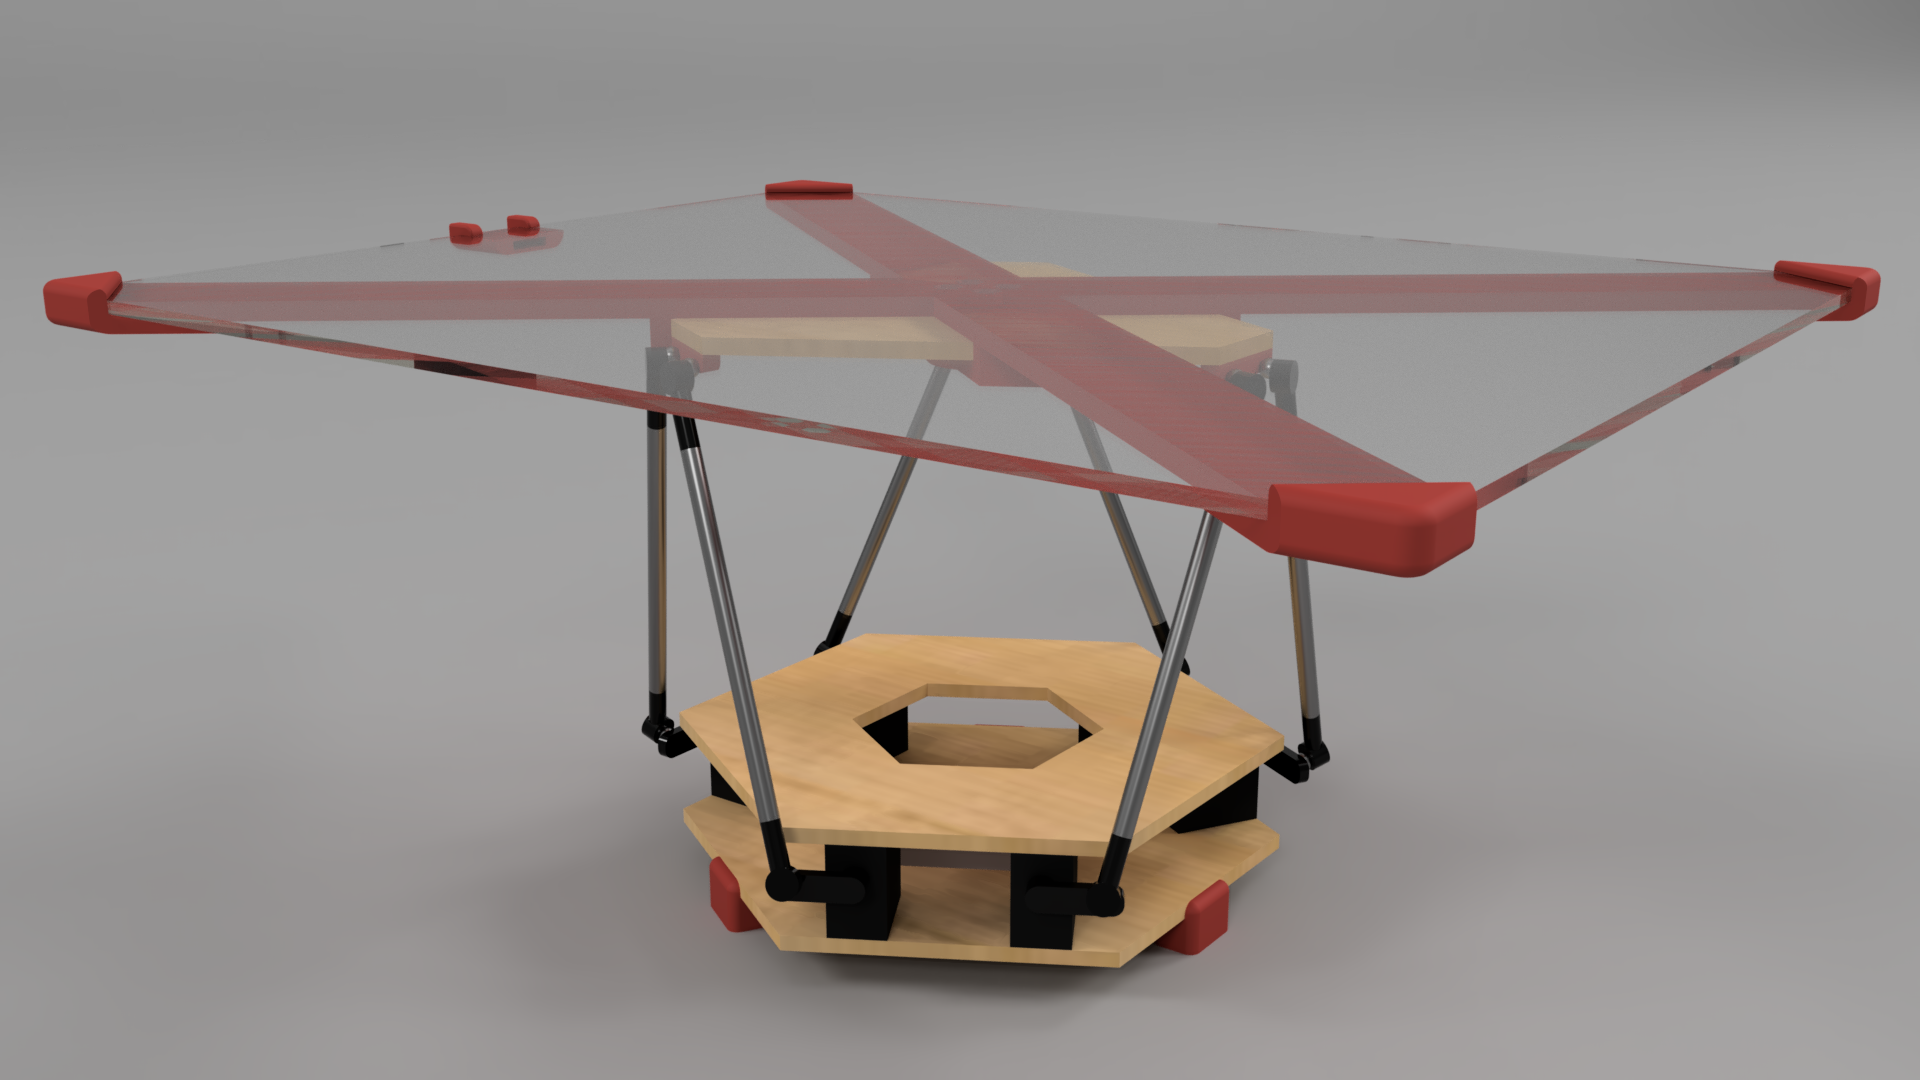
\includegraphics[width=\textwidth]{./images/stewart.png}
	\end{columns}
		%\end{block}
	\end{frame}
	
	\begin{frame}{Realizzazione Pratica}{Programmazione}

	
	\begin{itemize}
		\item Controllo semplice e intuitivo:\\ 
		\texttt{setPosition(x, y, z, rol, pit, yaw);}
		\item Controllo raggiungibilità posizione
		\item Implementazione controllore PID: 	\\
		\texttt{setPosition(0,0,108,radians(tiltX),radians(tiltY),radians(0));}
		\item Filtraggio dati
		\item Analisi all'oscilloscopio
		\item Programmazione figure di Lissajous
	\end{itemize}

	\end{frame}
	
	\begin{frame}{Realizzazione Pratica}{Programmazione}
	\centering\movie[width=12cm, height=6.75cm, poster, autostart, repeat]{}{./images/test.mp4}

	\end{frame}
	
	\begin{frame}[plain,noframenumbering]
	\standoutpage{\bfseries\huge Grazie per l'attenzione!}
	\end{frame}
	
	
	
	
	
	
	
	
	
	
	

	\section{Installation}
	\begin{frame}{Installation}
	The theme consists of five files
	\begin{enumerate}
		\item {\tt beamerthemeUniNA.sty}
		\item {\tt beamerinnerthemeUniNA.sty}
		\item {\tt beamerouterthemeUniNA.sty}
		\item {\tt beamercolorthemeUniNA.sty}
		\item {\tt beamerfontthemeUniNA.sty}
	\end{enumerate}
	The theme can either be installed for local or global use.
	\pause
	\begin{block}{Local Installation}
		The simplest way of installing the theme is by placing the five theme files in the same 
		folder as your presentation.
	\end{block}
	\end{frame}

	% general installation instructions
	\begin{frame}{Installation}
	\begin{block}{Global Installation}
	\begin{itemize}
		\item If you wish to make the theme globally available, you must put the files in your local LaTeX directory tree.
		The location of the root of the local directory tree depends on the operating system and the LaTeX distribution.
		\item Refer to your distribution's documentation for details.
	\end{itemize}
	\end{block}
	\end{frame}

\subsection{Required Packages}
% list of required packages
\begin{frame}{Installation}{Required Packages}
  Of course, you have to have the Beamer class installed. In addition, the theme loads the following packages:
  \begin{itemize}
	\item TikZ\footnote[frame]{By the way, TikZ is an awesome package for creating beautiful graphics, and this is a footnote.};
    \item calc, fp, adjustbox, setspace, transparent.
  \end{itemize}
  These packages are very common and should therefore be included in your LaTeX distribution.
\end{frame}
%%%%%%%%%%%%%%%%

\section{User Interface}
\subsection{Loading the Theme and Theme Options}
% list of the themes and options
\begin{frame}{User Interface}{Loading the Theme and Theme Options}
  \begin{block}{The Presentation Theme}
    It is very simple to load the presentation theme. Just type\\
    {\tt \textbackslash usetheme[<options>]\{UniNA\}}\\
	which is exactly the same way other beamer presentation themes are loaded. 
	The presentation theme loads the inner, outer, color and font UniNA theme files 
	and passes the {\tt <options>} on to these files.
  \end{block}
\end{frame}
%%%%%%%%%%%%%%%%

% list of the themes and options
\begin{frame}{User Interface}{Theme Options}
  \begin{block}{Theme options}
    The following options are available:
  \begin{itemize}
	\item {\tt rotationcw}: set the direction of the rotation of the progress circle 
	to clockwise instead of counterclockwise.
    \item {\tt sectionpages}: show section pages.
    \item {\tt logo}: used to specify the path to the logo to use in the upper right corner.
  \end{itemize}
  \end{block}
\end{frame}
%%%%%%%%%%%%%%%%

\subsection{Modifying the theme}
% how to modify the theme
{\setbeamercolor{UniNA}{fg=blue!50,bg=green!60}
 \setbeamercolor{structure}{fg=red}
 \setbeamercolor{frametitle}{use=structure,fg=structure.fg}
 \setbeamercolor{itemize/enumerate body}{fg=white, bg=red}
 \setbeamercolor{normal text}{fg=white}
 \setbeamercolor{alerted text}{fg=blue}
 \setbeamercolor{background canvas}{bg=purple!50}
\begin{frame}[fragile]{User Interface}{Modifying the Theme}
  \begin{itemize}[<+->]
	\item You can modify specific elements of the theme through the 
	templates provided by the beamer class. Please refer to the beamer user manual for instructions.
    \item For example, on this rather bizarre-looking slide the following commands have been used:
	\begin{verbatim}
\setbeamercolor{UniNA}{fg=blue!50,bg=green!60}
\setbeamercolor{structure}{fg=red}
\setbeamercolor{frametitle}{use=structure,fg=structure.fg}
\setbeamercolor{itemize/enumerate body}{fg=white, bg=red}
\setbeamercolor{normal text}{fg=white}
\setbeamercolor{alerted text}{fg=blue}
\setbeamercolor{background canvas}{bg=purple!50}
	\end{verbatim}
  \end{itemize}
\end{frame}
}

\begin{frame}{User Interface}{Modifying the Theme}
	\begin{itemize}[<+->]
		\item If you want to change the main colour and need a matching Federico II logo,
		  	you can compile your own as follows:
		  	\begin{enumerate}[<+->]
				\item change the definition of \texttt{logocolor} in 
					\texttt{logo/logo-federico-II.tex} accordingly to your needs;
				\item compile \texttt{logo/logo-federico-II.tex} with \texttt{xelatex};
			\end{enumerate}
		\item With your version of the logo in place, you can change the value of the \texttt{logo}
			parameter to the path of your own logo.
	\end{itemize}
\end{frame}

\subsection{Frames}

\begin{frame}[plain]{Plain frame}{Subtitle}
	This is a frame with no header thanks to the \texttt{plain} option.
\end{frame}

\begin{frame}[noframenumbering]{Unnumbered frame}{Subtitle}
	This is a frame not contributing to the frame count, thanks to the \texttt{noframenumbering} option.
\end{frame}

\subsection{Math and blocks}

\begin{frame}{Math and blocks}{Test math and blocks}
	The following text is \alert<2>{alerted} in the next slide. 
	Now some math mode:
	if $R=\{x\mid x\not\in x\}$, then $R\in R \Leftrightarrow R\not\in R$.
	\begin{block}{Observation}
	This is an observation.
	\end{block}
	\begin{exampleblock}{Example 14}
	This is a nice example block.
	\end{exampleblock}
	\begin{alertblock}{Beware!}
	Naive set theory is \emph{a wolf in sheep's clothing?}
	\end{alertblock}
\end{frame}

\subsection{Standout frames}


\begin{frame}[fragile]{Standout frames}{}
	The UniNA beamer theme supports standout frames. For example, the following
	\begin{verbatim}
\begin{frame}[plain,noframenumbering]
	\standoutpage{This is a dark standout frame!}
\ end{frame}

\begin{frame}[plain,noframenumbering]
	\standoutpagelight{This is a light standout frame!}
\ end{frame}
	\end{verbatim}
	produces the following two slides.
\end{frame}

\begin{frame}[plain,noframenumbering]
	\standoutpage{This is a dark standout frame!}
\end{frame}

\begin{frame}[plain,noframenumbering]
	\standoutpagelight{This is a light standout frame!}
\end{frame}

\subsection{Widescreen Support}
% Widescreen Support
\begin{frame}{User Interface}{Widescreen Support}
\begin{block}{Widescreen Support}
	Newer projectors and almost any modern TV support a widescreen format such as 16:10 or 16:9. Beamer (>= v. 3.10) supports various aspect ratios of the slides. According to section 8.3 on page 77 of the Beamer user guide v. 3.10, you can write\\
{\tt\textbackslash documentclass[aspectratio=1610]\{beamer\}}\\
to get slides with an aspect ratio of 16:10. You can also use 169, 149, 54, 43 (default), and 32 to get other aspect ratios.
\end{block}
\end{frame}

%final slide
\begin{frame}[plain,noframenumbering]
	\standoutpage{\bfseries\huge Thank you for your time!}
\end{frame}

\end{document}
		